\section{Summary LSTM \cite{Vlachas}}

	The invention of LSTM was motivated by the regularization of recurrent neural networks (RNNs). In addition to inputs $\bm{i}_t \in \mathbb{R}^{d_i}$, RNNs use also loops in order to include informations from previous hidden states $\bm{h}_{t'}$(where $t'<t$) in the calculation of the current state $\bm{h}_t \in \mathbb{R}^{d_h}$ at time $t$. The Elman network \cite{Elman} is for example defined by \footnote{see also \url{https://en.wikipedia.org/wiki/Recurrent_neural_network\#Elman_networks_and_Jordan_networks}}:
	\begin{figure}[h]
	\begin{minipage}[h][3cm][t]{7cm}
	\begin{align}
		\bm{h}_t&=\sigma_h(\bm{W}_{hi}\cdot\bm{i}_t+\bm{W}_{hh}\cdot\bm{h_{t-1}}+\bm{b}_h)\\
		\bm{o}_t&=\sigma_o(\bm{W}_{oh}\cdot\bm{h}_t+\bm{b}_o) \in \mathbb{R}^{d_o} \quad \footnotemark
	\end{align}
	\vfill
	\caption{Schematic Sketch of a RNN \cite{Vlachas}}
	\end{minipage}
	\begin{minipage}[h][3cm][c]{7.5cm}
		\centering
		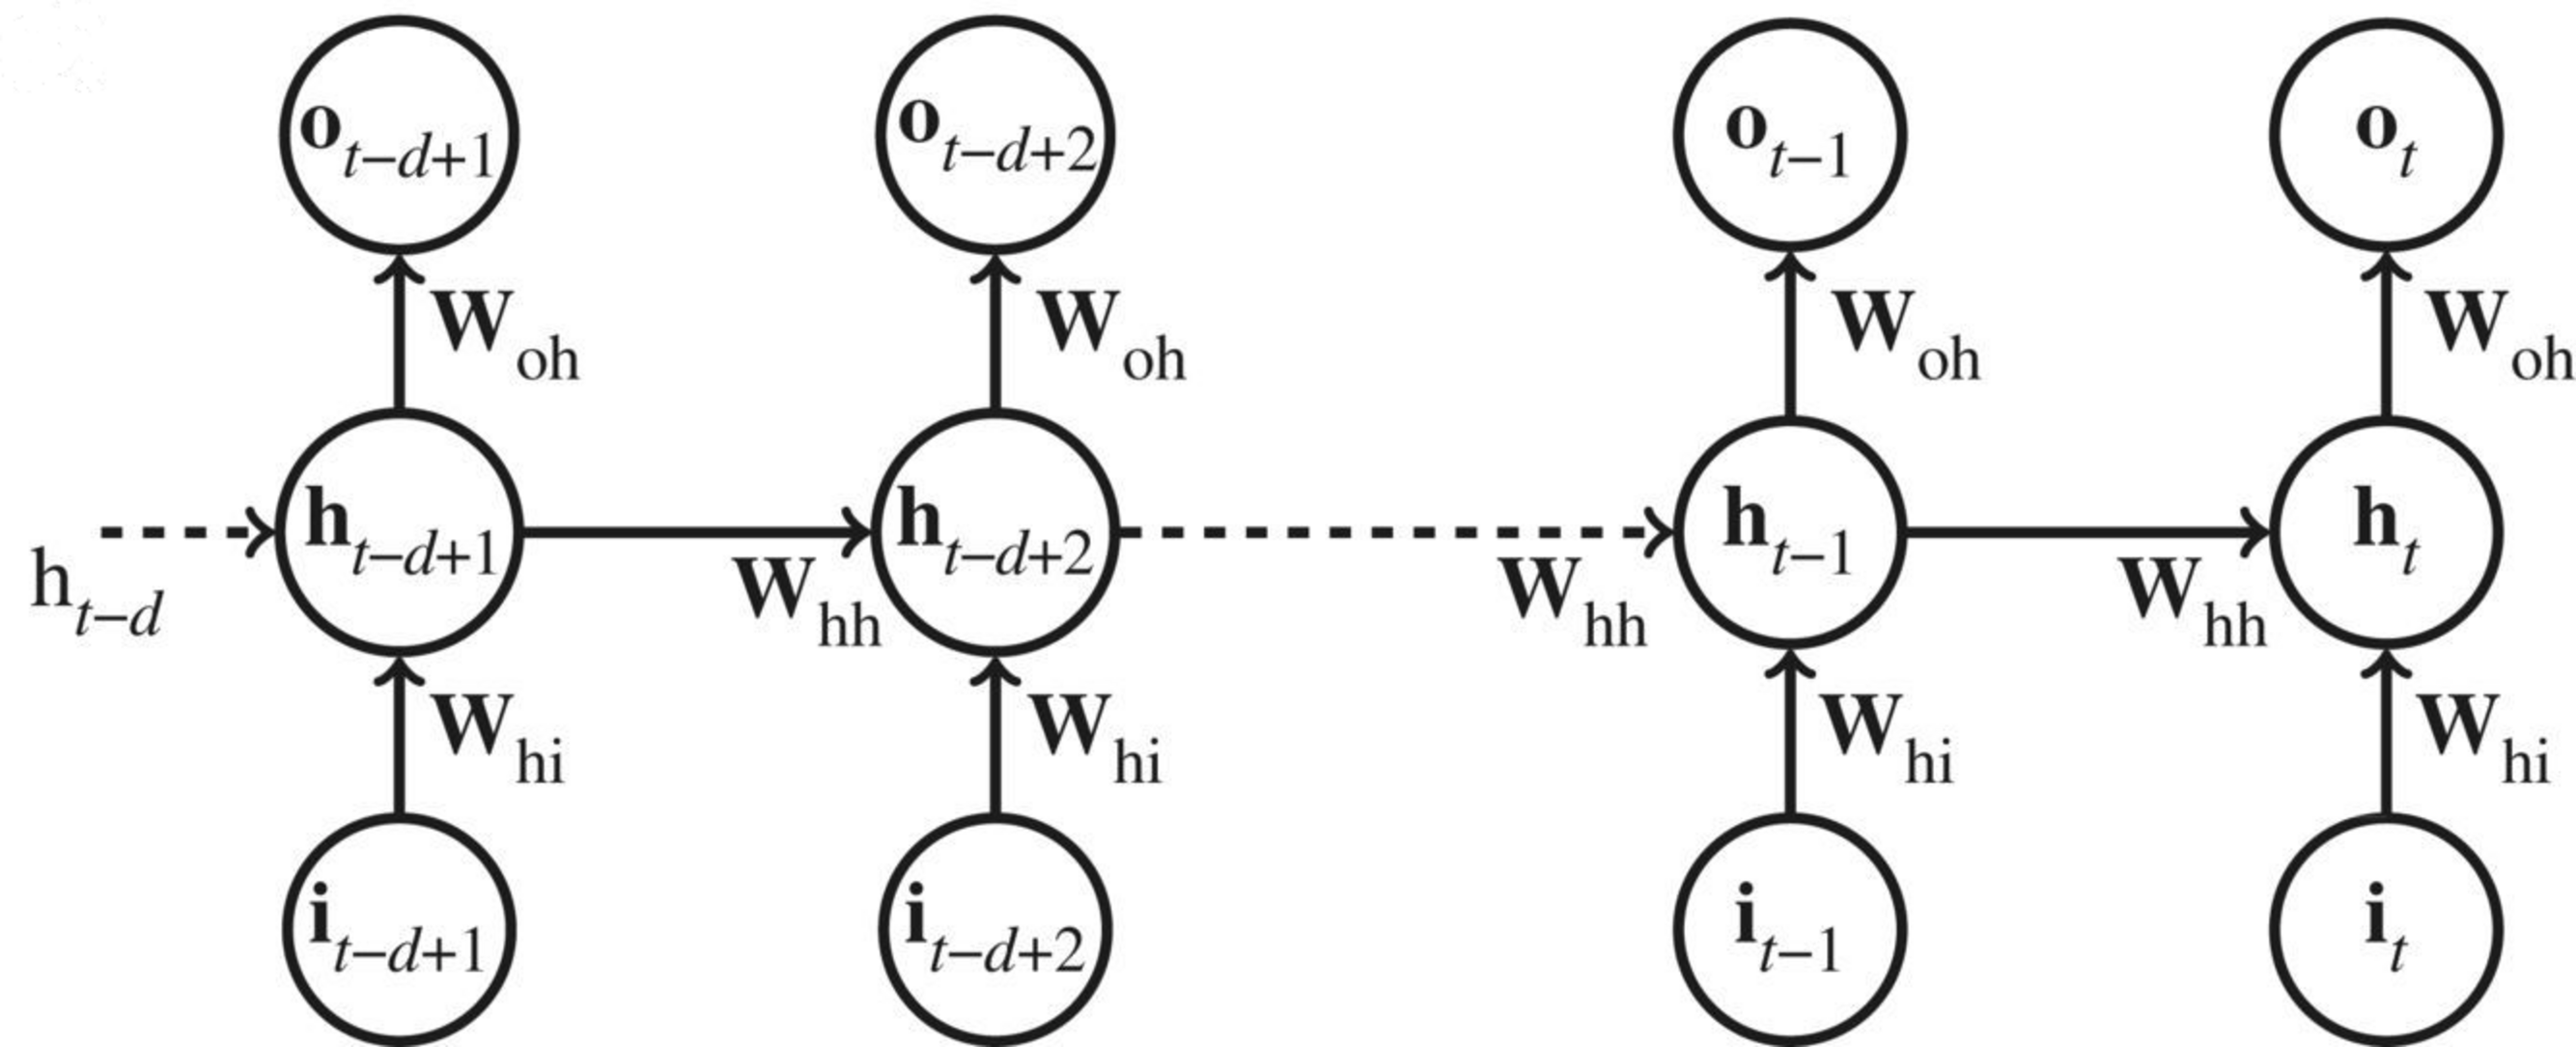
\includegraphics[width=7.3cm]{images/RNN_Vlachas_cropped.png}
	\end{minipage}
	\end{figure}
	\footnotetext{where $\sigma_\bullet$ are activation functions, $\bm{W}_{*\bullet}$ weight matrices and $\bm{b}_\bullet$ bias summands.}
	However RNNs struggle to recognize long-term dependencies and furthermore the gradient can vanish or explode, which also leads to problems. Because of this one uses gates. The corresponding model is called LSTM (Long Short-Term Memory). This is characterised by the following formula:
	\begin{equation}
	\begin{aligned}
		&\bm{g}^f = \sigma_f(\bm{W}_f\cdot[\bm{h}_{t-1}, \bm{i}_t]+\bm{b}_f)\\
		&\tilde{\bm{C}}_t = \text{tanh}(\bm{W}_C\cdot[\bm{h}_{t-1}, \bm{i}_t]+\bm{b}_C)\\
		&\bm{g}_t^o=\sigma_h(\bm{W}_h\cdot[\bm{h}_{t-1}, \bm{i}_t]+\bm{b}_h)
	\end{aligned}
	\quad
	\begin{aligned}
		&\bm{g}_t^i=\sigma_i(\bm{W}_i\cdot[\bm{h}_{t-1}, \bm{i}_t]+\bm{b}_i)\\
		&\bm{C}_t = \bm{g}_t^f\cdot\bm{C}_{t-1} +\bm{g}_t^i\cdot\tilde{\bm{C}}_t\\
		&\bm{h}_t = \bm{g}_t^o\cdot\text{tanh}(\bm{C}_t)
	\end{aligned}
	\end{equation}
	Whereby $\bm{g}_\bullet\in\mathbb{R}^{d_h\times(d_h+d_i)}$ represents the gate signal and $\bm{C}_t\in\mathbb{R}^{d_h}$ the so-called cell state, which is jointly with the hidden state referred as "LSTM states". To map the hidden state to the wanted output space one also uses an additional fully connected layer $\bm{W}_{oh}$:
	\begin{align}
		\bm{o}_t = \bm{W}_{oh}\cdot\bm{h}_t = f^w(\bm{z}_t, \bm{h}_{t-1}, \bm{C}_{t-1}) \approx F^w(\bm{z}_t, \bm{z}_{t-1}, \hdots, \bm{z}_{t-d+1}) \quad\footnotemark
	\end{align}
	\footnotetext{where in the following $\bm{z}_t$ is used as the input and describes the system time series.} 
	The so-called LSTM cell-function $f^w$ can be rewritten by iterative repition as $F^w$, where $w$ includes all trainable parameters. In the last step one uses the assumption that d-time steps are sufficient to compute the current output and thus $\bm{h}_{t-d},\bm{C}_{t-d}$ can be omitted. The model is data-driven, one has not to incoperate prior knowledge (like underlying equations) in the system necessarily.
	Goal of the LSTM is to predict the state derivative $\bm{\dot{z}}_t$ using a short time memory of the $d$ previous states $\bm{z}_{t:t-d+1}$. Therefore, the loss $\mathcal{L}$ shall be minimized by searching for the best parameters $w^*$:
	\begin{align}
	w^* = \arg\min_w\mathcal{L}(\{\bm{z}_{1:T},\bm{\dot{z}}_{1:T}\},w)=\arg\min_w\frac{1}{T-d+1}\sum_{t=d}^T||F^w(\bm{z}_{t:t-d+1})-\bm{\dot{z}}_t||^2
	\end{align}
	\begin{SCfigure}
		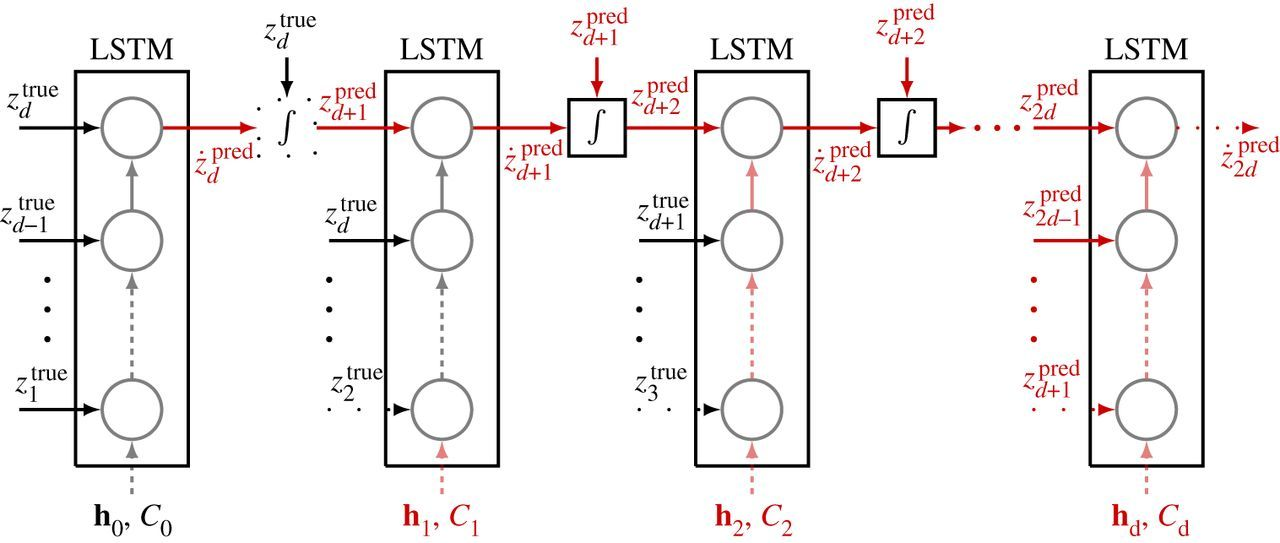
\includegraphics[width=9.25cm]{images/LSTM_Vlachas.jpg}
		\captionsetup{format=plain}
		\caption{LSTM Model\cite{Vlachas}\\Predictions are marked with red arrows, while black arrows indicate the short-term memory. The known $\bm{z}_{1:d}^{\text{true}}$ are used to predict $\bm{\dot{z}}_d^{\text{predict}}$, which can be integrated in order to get the next state $\bm{z}_{d+1}^{\text{predict}}$.}
	\end{SCfigure}

	The group of Vlachas trained the LSTM by using backpropagation. For this, a mini-batch optimization with the Adam method \cite{Adam} and an initial learning rate $\epsilon_{init}=10^{-4})$ was applied. The inizialization of the weights is based on the method of Xavier. One problem the group had to face was to fine tune the dimension of the hidden stated $d_h$. They observed that a small $d_h$ shortened the ability to fit to the time series well, but a big $d_h$ increased the risk of overfitting and the computation time.
	
	In the paper they compared the LSTM Model with the GPR (Gaussian process regression) and MSM (Mean Stochastic Model). Three applications (The Lorenz 96 sytem, the Kuromoto-Sivashinsky equation an a barotropic climate model) were considered in order to evaluate the predictive accuracy of the models. They showed that in all cases the LSTM outperformed the other two models, i.e. the LSTM model was able to catpure the local dynamics more efficient.